%%%%%%%%%%%%%%%%%%%%%%%%%%%%%%%%%%%%%%%%%%%%%%%%
% E.Pinault-Bigeard - e.pinault-bigeard@upsti.fr
% http://s2i.pinault-bigeard.com
% CC BY-NC-SA 2.0 FR - http://creativecommons.org/licenses/by-nc-sa/2.0/fr/
%%%%%%%%%%%%%%%%%%%%%%%%%%%%%%%%%%%%%%%%%%%%%%%%
\documentclass[11pt]{article}
%%%%%%%%%%%%%%%%%%%%%%%%%%%%%%%%%%%%%%%%%%%%%%%%
% Package UPSTI_Document
%%%%%%%%%%%%%%%%%%%%%%%%%%%%%%%%%%%%%%%%%%%%%%%%
\usepackage{subcaption}
\usepackage[usenames, svgnames, dvipsnames]{xcolor}
\usepackage{UPSTI_Document}
\definecolor{darkspringgreen}{rgb}{0.09, 0.45, 0.27}

%---------------------------------%
% Paramètres du package
%---------------------------------%

% Version du document (pour la compilation)
% 1: Document prof
% 2: Document élève
% 3: Document à publier
\newcommand{\UPSTIidVersionDocument}{1}

% Variante
%\newcommand{\UPSTIvariante}{2}

% Classe
% 1: PTSI				6: PSI*			11: TSI2		16: Spé
% 2: PT	(par défaut)	7: MPSI			12: ATS
% 3: PT*				8: MP			13: PC
% 4: PCSI				9: MP*			14: PC*
% 5: PSI				10: TSI1		15: Sup
%\newcommand{\UPSTIidClasse}{2}

% Affichage personnalisé de la classe
\newcommand{\UPSTIclasse}{Première STI2D}

% Matière
% 1: S2I (par défaut)    2: IPT     3: TIPE
% 6: Vie au lycée
\newcommand{\UPSTIidMatiere}{4}

% Type de document
% 0: Custom*				7: Fiche Métho de			14: Document Réponses
% 1: Cours (par défaut)		8: Fiche Synthèse    		15: Programme de colle
% 2: TD     				9: Formulaire
% 3: TP						10: Memo
% 4: Colle					11: Dossier Technique
% 5: DS						12: Dossier Ressource
% 6: DM						13: Concours Blanc
% * Si on met la valeur 0, il faut décommenter la ligne suivante:
%\newcommand{\UPSTItypeDocument}{Custom}
\newcommand{\UPSTIidTypeDocument}{1}

% Titre dans l'en-tête
\newcommand{\UPSTItitreEnTete}{Communiquer}
%\newcommand{\UPSTItitreEnTetePages}{UPSTItitreEnTetePages}
%\newcommand{\UPSTIsousTitreEnTete}{UPSTIsousTitreEnTete}

% Titre
%\newcommand{\UPSTItitrePreambule}{Qu'est-ce qu'un réseau ?}
\newcommand{\UPSTItitre}{Vous êtes-vous déjà demandé comment ça fonctionne ?}

% Durée de l'activité (pour DS, DM et TP)
\newcommand{\UPSTIduree}{1h}

% Note de bas de première page
%\newcommand{\UPSTInoteBasDePremierePage}{Note de bas de 1ère page}
% Numéro (ajoute " n°1" après DS ou DM)
%\newcommand{\UPSTInumero}{1}

% Numéro chapitre
\newcommand{\UPSTInumeroChapitre}{5}

% En-tête customisé
%\newcommand{\UPSTIenTetePrincipalCustom}{UPSTIenTetePrincipalCustom}

% Message sous le titre
%\newcommand{\UPSTImessage}{Message sous le titre}

% Référence au programme
%\newcommand{\UPSTIprogramme}{\EPBComp \EPBCompP{B1-02}, \EPBCompP{B2-49}, \EPBCompS{B2-50}, \EPBCompS{B2-51}, \EPBCompP{C1-07}, \EPBCompP{C1-08}}

% Si l'auteur n'est pas l'auteur par défaut
%\renewcommand{\UPSTIauteur}{WWOOOOOOWW}

% Si le document est réalisé au nom de l'équipe
%\newcommand{\UPSTIdocumentCollegial}{1}

% Source
%\newcommand{\UPSTIsource}{UPSTI}


% Version du document
\newcommand{\UPSTInumeroVersion}{1.0}

%-----------------------------------------------
\UPSTIcompileVars		% "Compile" les variables
%%%%%%%%%%%%%%%%%%%%%%%%%%%%%%%%%%%%%%%%%%%%%%%%


%%%%%%%%%%%%%%%%%%%%%%%%%%%%%%%%%%%%%%%%%%%%%%%%
% Début du document
%%%%%%%%%%%%%%%%%%%%%%%%%%%%%%%%%%%%%%%%%%%%%%%%
\begin{document}
\UPSTIbuildPage

\section{Pourquoi et comment communiquer ?}
De tout temps, les humains ont ressenti et ressentent le besoin de communiquer.
Les méthodes dont nous nous servons pour partager idées et informations changent et évoluent sans cesse. Si le réseau humain se limitait autrefois à des conversations en face à face, aujourd'hui les découvertes en matière de supports étendent sans cesse la portée de nos communications. De la presse écrite à la télévision, chaque innovation a développé et amélioré nos moyens de communication.

\section{Caractéristiques d'un réseau}
\label{sec:caracteristiques}
Pour être totalement fonctionnels et répondre aux besoins des utilisateurs, les réseaux doivent respecter quelques caractéristiques que nous décrivons dans cette section.


\subsection{Tolérence aux pannes}
La fréquence d'utilisation et la taille des réseaux soumettent les services disponibles en réseau à diverses pannes matérielles et/ou logicielles.
\UPSTIdefinition{
  Un réseau tolérant aux pannes est un réseau qui limite l'impact des pannes du matériel et des logiciels et qui peut être rétabli rapidement quand des pannes se produisent.
}
\UPSTIexemple{
  Pour pallier à des pannes de laison entre deux organes du réseau, on peut mettre en place une redondance entre la source et la destination. Cela signifie qu'il y aura plusieurs chemins possibles pour joindre la destination depuis la source.
  En cas de défaillance d'une liaison (ou chemin) entre deux hôtes, des processus s'assurent que les messages sont routés (dirigés) sur un chemin différent et arrivent à bon port.
  \begin{center}
    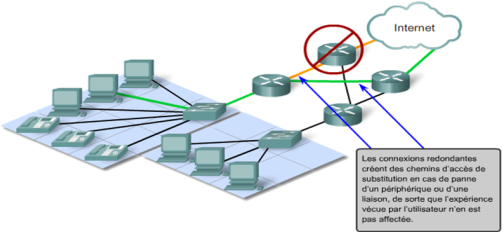
\includegraphics[width=.7\textwidth]{Src/Images/reseau_redondances}
  \end{center}
}

\subsection{Evolutivité}
Le nombre croissant d'utilisateurs d'internet, l'évolution imprévisible d'une entreprise ou d'un organisme ou encore l'arrivée de matériel spécifique impose une évolution du réseau afin qu'il puisse répondre aux nouveaux besoins.
\UPSTIdefinition{
  Un réseau évolutif est en mesure de s'étendre rapidement afin de prendre en charge de nouveaux utilisateurs et de nouvelles applications sans que cela n'affecte les performances du service fourni aux utilisateurs existants.
}

\subsection{Qualité de services}
Les transmissions exigent des niveaux de qualités différents selon l'information qui circule. Par exemple, une transmission audio et vidéo exige un service ininterrompu et une qualité supérieure à l'envoi d'un simple mail.
\UPSTIaRetenir{
  Sur un réseau, un niveau de priorité est défini pour chaque service en fonction de la qualité requise. Ainsi, plus un service exige une qualité importante, plus ses paquets seront prioritaires devant d'autre services.
  \begin{center}
    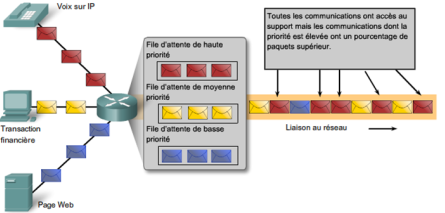
\includegraphics[width=.8\textwidth]{Src/Images/reseau_priorites}
  \end{center}
}

\subsection{Sécurité}
En matière de sécurité des réseaux, deux points doivent être pris en considération pour éviter des conséquences graves : la sécurité de l'infrastructure réseau et la sécurité du contenu.
En effet, les données qui transitent sur un réseau peuvent être plus ou moins sensibles (données bancaires par exemple) et doivent donc pouvoir être transmises en garantissant une certaine sécurité.
Le réseau peut également subir des attaques malveillantes visant à le rendre hors service.
\UPSTIaRetenir{~
  \begin{itemize}
    \item \textbf{Sécuriser l'infrastructure} réseau implique de {sécuriser matériellement et logiquement les périphériques qui assurent la connectivité du réseau} et d'empêcher tout accès non autorisé au logiciel de gestion qu'ils hébergent.
    \item \textbf{Sécuriser le contenu} consiste à protéger {les informations contenues dans les paquets transmis sur le réseau} ainsi que les informations stockées sur des périphériques reliés au réseau en les cryptant.
  \end{itemize}
}
\section{Elements d'un réseau}
\begin{figure}[h!t]
  \centering
  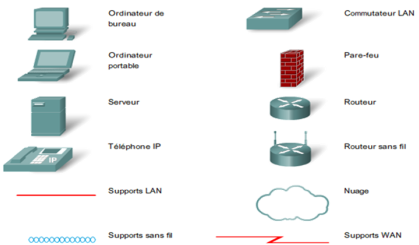
\includegraphics[height=.3\textheight]{Src/Images/reseau_peripheriques}
  \caption{Périphériques et supports de transmissions}
\end{figure}

\subsection{Les périphériques terminaux}
\UPSTIdefinition{
  Les périphériques terminaux sont ceux qui envoient ou auxquels sont destinés les infomations transitant sur le réseau.
}
\UPSTIexemple{~\\
  \begin{minipage}[c]{.5\textwidth}
    \begin{itemize}
      \item {Serveurs}
      \item {Ordinateurs}
      \item {Imprimantes}
      \item {Téléphones IP}
    \end{itemize}
  \end{minipage}
  \begin{minipage}[c]{.5\textwidth}
    \begin{itemize}
      \item {Smartphones}
      \item {Tablettes}
      \item {Télévisions}
      \item \dots
    \end{itemize}
  \end{minipage}
}
\subsection{Les périphériques intermédiaires}
\UPSTIdefinition{
  Ces périphériques assurent le bon acheminement des paquets sur le réseau tout en garantissant le respect des caractéristiques explicités dans la section~\ref{sec:caracteristiques}
}
\UPSTIexemple{~\\
    \begin{itemize}
      \item {Commutateurs (utilisés pour interconnecter des réseaux locaux)}
      \item {Pare-feu (assure la sécurité du réseau)}
      \item {Routeur (contribue à orienter les messages transitant sur un réseau)}
      \item {Routeur sans fils (souvent présents dans les réseaux domiciles)}
      \item \dots
    \end{itemize}
}
\subsection{Les connexions}
\UPSTIdefinition{
  Les connexions sont le support même du transfert d'informations. Ces connexions peuvent être filaires, sans-fil, optiques ou tout support capable de transporter une information.
}
Divers organismes de normalisation contribuent à la définition des propriétés physiques, électriques et mécaniques des supports disponibles pour différentes communications de données.
Ces spécifications garantissent que les câbles et connecteurs fonctionnent comme prévu dans des conditions précises.


\section{Topologies des réseaux}
Afin de permettre à des éléments de communiquer, il est indispensable de les connecter entre eux. Il existe une multitude de connexions possibles.
\UPSTIdefinition{
  La \textbf{topologie physique} désigne la configuration spatiale du réseau. C'est la façon dont les organes sont connectés \textbf{physiquement}.
}
\UPSTIdefinition{
  La \textbf{topologie logique} désigne quant à elle la manière dont les données transitent dans les câbles.
}

\subsection{Quelques topologies physiques classiques}
\begin{figure}[h!t]
  \centering
  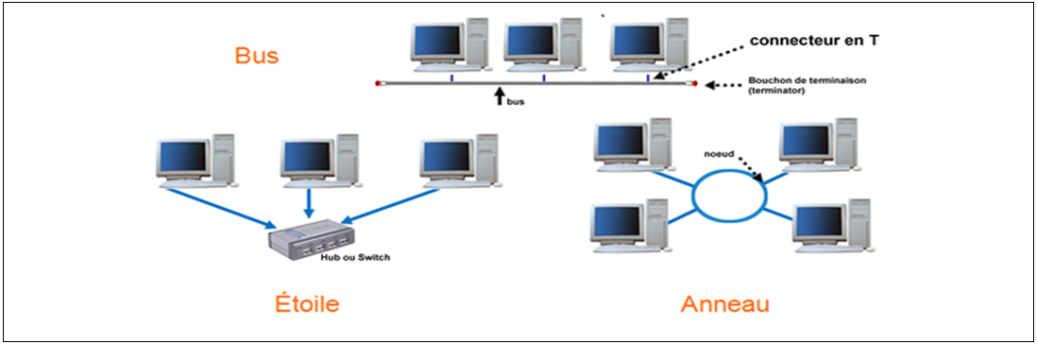
\includegraphics[width=.7\textwidth]{Src/Images/reseau_topologies}
  \caption{Trois exemples de topologies de réseau.}
  \label{fig:res_topo}
\end{figure}
\subsubsection{Topologie en bus}
Une topologie en bus est l'organisation la plus simple d'un réseau. En effet dans une topologie en bus tous les ordinateurs sont reliés à une même ligne de transmission par l'intermédiaire d'un câble, généralement coaxial. Le mot "bus" désigne la ligne physique qui relie les machines du réseau.

Cette topologie a pour avantages d'être {facile à mettre en oeuvre} et de fonctionner facilement, par contre elle est extrêmement {vulnérable} étant donné que si l'une des connexions est défectueuse, c'est l'ensemble du réseau qui est affecté.

Cette topologie est obsolète dans les réseaux de données mais couramment utilisé dans les réseaux de terrain (voitures ou automates par exemple).

\subsubsection{Topologie en anneau}
Dans un réseau en topologie en anneau, les ordinateurs sont reliés sur une bouble. Les ordinateurs doivent donc communiquer chacun à leur tour.

En réalité les ordinateurs d'un réseau en topologie anneau ne sont pas reliés en boucle, mais sont reliés à un répartiteur (appelé MAU, Multistation Access Unit) qui va gérer la communication entre les ordinateurs qui lui sont reliés en impartissant à chacun d'entre-eux un temps de parole.

\subsubsection{Topologie en étoile}
Dans une topologie en étoile, les ordinateurs du réseau sont reliés à un système matériel appelé switch (commutateur). Il s'agit d'une boîte comprenant un certain nombre de jonctions auxquelles on peut connecter les câbles en provenance des ordinateurs. Celui-ci a pour rôle d'assurer la communication entre les différentes jonctions.
C'est la topologie la plus utilisée aujourd'hui.

Contrairement aux réseaux construits sur une topologie en bus, les réseaux suivant une topologie en étoile sont beaucoup moins vulnérables car on peut aisément retirer une des connexions en la débranchant du commutateur sans pour autant paralyser le reste du réseau.

\section{Le modèle OSI}
Au début des années 70, chaque constructeur a développé sa propre solution réseau autour d'architecture et de protocoles privés (SNA d'IBM, DECnet de DEC, DSA de Bull, TCP/IP du DoD,...) et il s'est vite avéré qu'il serait impossible d'interconnecter ces différents réseaux «propriétaires» si une norme internationale n'était pas établie. Cette norme établie par l'International Standard Organization (ISO) est la norme Open System Interconnection (OSI, interconnexion de systèmes ouverts).

Un système ouvert est un ordinateur, un terminal, un réseau, n'importe quel équipement respectant cette norme et donc apte à échanger des informations avec d'autres équipements hétérogènes et issus de constructeurs différents.

Le modèle de référence OSI est une représentation abstraite en couches servant de guide à la conception des protocoles réseau. Il divise le processus de réseau en sept couches logiques, chacune comportant des fonctionnalités uniques et se voyant attribuer des services et des protocoles spécifiques.

\begin{figure}[h!t]
  \centering
  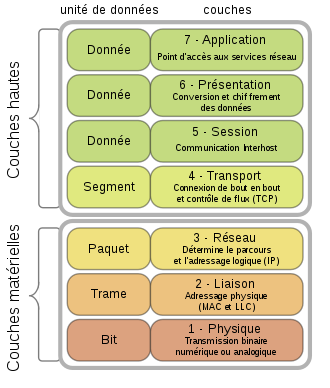
\includegraphics[height=.3\textheight]{Src/Images/reseau_OSI}
  \caption{Les couches du modèle OSI}
  \label{fig:res_osi}
\end{figure}

\section{Adressage et encapsulation}
\paragraph{Nécessité d'un adressage}
Lorsque deux organes sont connectés entre eux seuls, il est simple de savoir qui s'adresse à qui (il n'y a qu'un seul expéditeur et un seul destinataire possible selon le sens de communication).
Par contre, lorsque plusieurs organes sont connectés sur le même réseau, il devient indispensable de savoir à qui s'adresse chaque paquet qui transite sur le réseau.
\paragraph{}
Le modèle OSI décrit des processus de codage, de mise en forme, de segmentation et d'encapsulation de données pour la transmission sur le réseau. Un flux de données envoyé depuis une source vers une destination peut être divisé en parties et entrelacé avec des messages transmis depuis d'autres hôtes vers d'autres destinations. À n'importe quel moment, des milliards de ces parties d'informations se déplacent sur un réseau. Il est essentiel que chaque donnée contienne les informations d'identification suffisantes afin d'arriver à bonne destination.

Il existe plusieurs types d'adresses qui doivent être incluses pour livrer correctement les données depuis une application source exécutée sur un hôte à l'application de destination correcte exécutée sur un autre. En utilisant le modèle OSI comme guide, nous apercevons les différents identificateurs et adresses nécessaires à chaque couche.

\subsection{Protocole TCP/IP et analogies utiles}
On s'interesse dans cette partie aux couches 1 à 4 du réseau plus particulièrement. Ces couches permettent d'adressser et d'orienter un message vers la bonne application du bon destinataire. Les couches supérieures seront ici considérées comme un paquet de données.

Tout au long de cette section, une analogie sera faite avec l'envoi d'un courrier à une personne dans une entreprise.

\begin{figure}[h!t]
  \centering
  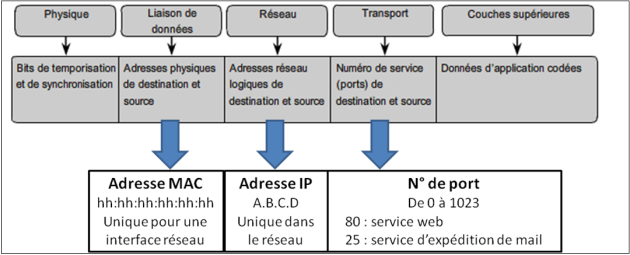
\includegraphics[width=.7\textwidth]{Src/Images/reseau_couches_adressage}
  \caption{Principe de l'encapsulation des données}
  \label{fig:res_encap_generique}
\end{figure}

\subsubsection{Les couches supérieures}
Les couches supérieures (5 à 7) concernent les données, le message en tant que tel. Il s'agit donc {du contenu qui doit arriver à bon port.}
\UPSTIremarque{
  Dans notre analogie, il s'agit ici du contenu de la lettre que nous souhaitons envoyer.
}

\subsubsection{La couche de transport (TCP)}
Cette couche détermine à quel service (port) {s'adressent les données}. Par exemple, par convention les données concernant les pages WEB sont envoyées sur le port 80 d'une machine.

\UPSTIremarque{
  Dans notre analogie, il s'agit ici du service auquel nous nous adressons dans l'entreprise ou l'organisation (gestion des compte cantine des élèves par exemple).
}

\subsubsection{La couche réseau (protocole IP)}
Cette couche détermine {où doit être acheminée le paquet de données sur le réseau}. L'adresse IP est un identifiant unique sur le réseau permettant d'orienter le paquet vers le destinataire du message.

\UPSTIremarque{
  Dans notre analogie, il s'agit de l'adresse que l'on écrira sur l'enveloppe.
}

\subsubsection{La couche Trame (adresse MAC)}
L'adresse MAC identifie, de manière \textbf{unique} dans le monde, la machine destinatrice du message.

\UPSTIremarque{
  Dans notre analogie, il s'agit de la personne précise s'occupant de la requête. On peut voir l'adresse IP comme l'identifiant de sécurité sociale, unique en France.
}

\subsubsection{La couche physique}
Il s'agit ici de la façon pour les données de transiter sur le réseau (bits de temporisation, synchronisation des signaux, \textit{etc.})

\UPSTIremarque{
  Dans notre analogie, ce serait le service de courrier en lui même, avec son architecture d'acheminement (camions, centre de tri, \dots)
}

\subsection{L'encapsulation des données}
Toutes les informations présentées dans la partie précédentes sont indispensables au bon acheminement d'un paquet. De la même façon qu'un courrier est encapsulé dans une enveloppe sur laquelle sont écrites les informations d'adressage, les paquets internet sont encapsulé dans un message de la couche supérieur contenant les informations indispensables (voir Figure~\ref{fig:res_encapsulation}).

\begin{figure}[h!t]
  \centering
  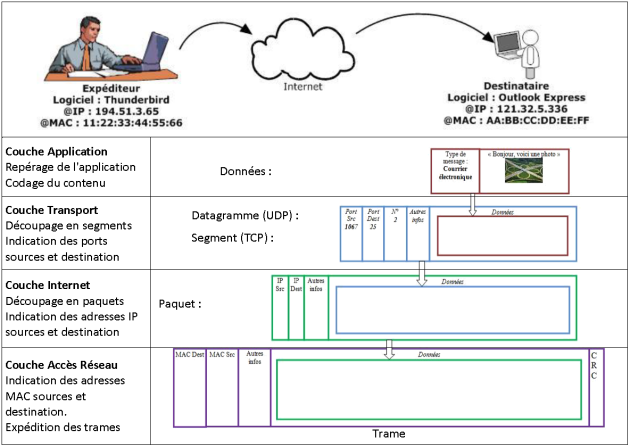
\includegraphics[width=.7\textwidth]{Src/Images/reseau_encapsulation}
  \caption{Exemple d'encapsulation de données}
  \label{fig:res_encapsulation}
\end{figure}

\end{document}
